\section{BuyBox Prediction}
\label{sec:buybox}
% This is the brief introduction of our goal in this section
This section provides a machine learning algorithm that can be trained on historical data from the Amazon, to predict the winner of an auction on the marketplace. This algorithm can take as input any dataset describing the offers made by sellers for a set of products, for a specific market (e.g., US, UK, France) or across markets. It then trains for each marketplace a machine learning model, which can predict the offer that will win the auction (BuyBox). The algorithm also outputs a ranked list of the feature importance discovered from the training data. For example, the algorithm can discover data-specific feature importance for each input dataset. This means that the algorithm can be targeted to the data of a single seller or a specific product, and it delivers a list of feature importance for that custom data. So besides predicting the auction winner, the algorithm can be used to advise sellers on how best to update their offer profiles to increase their chance of winning the BuyBox.

\subsection{Business Understanding}
\label{sec:bbbusiness}
%% our target in increasing profit by placing offer into BuyBox
Amazon hosts thousands of  sellers on their marketplace. They use an algorithmic decision process to decide the winner of every auction. An auction as mentioned above is a set of merchants that compete to sell a product. Amazon selects a winner for the auction, and place that seller's product into the BuyBox. The BuyBox winner typically sells more products, and ideally achieves a higher profit margin. This means that the winner is highly competed by many retailers in auction.

Motivated by that, our target is clearly declared as: can we use historical data about auctions and knowledge about the winners and losers, to learn the rules by which Amazon decides the winners? If we can approximate Amazon’s algorithm, we can advise sellers about the best strategy to use for winning the BuyBox. For example, we can recommend a new price for the product, or give advice about shipping time and user feedback profile to improve the offer and increase the chance of winning the BuyBox. 

\subsection{Data Understanding}
\label{sec:datafirstlook}
% Scale of amazon data
As mentioned above, every changing for a seller's offer detail in product page provides an auction, in AWS cloud. It includes aggregated information about the 20 lowest prices offered for a product (or less, if there are less than 20 sellers). Each auction is represented as a XML, the total size of raw-data folder, which is a cross-market database, is about 100.000 files. 
\begin{figure}[!h]
	\begin{center}
		\scalebox{0.5}{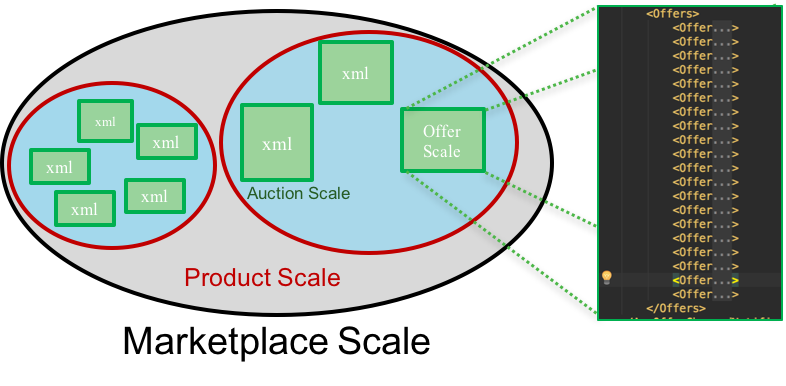
\includegraphics{fig3_scale.png}}
	\end{center}
	\caption{\label{fig:scale}The scales of data in one Marketplace.}
\end{figure}

Illustrating from \textbf{Fig.\ref{fig:scale}},which is the scaling scheme of data in one market, there are four basic layer for the Amazon data:

1. \textbf{Marketplace layer}: The Amazon has many marketplaces for
the United States, Australia, Brazil, Canada, China, France, Germany, India, Italy, Japan, Mexico, Netherlands, Spain, and the United Kingdom. One marketplace is an separated  environment with its own characteristics.  e.g. in India market, there is one seller who wins almost product's competing, while in U.S. market, the auction is normally with two or three competitors.

2. \textbf{Product layer}: From the market place, sellers can sell many products. It could be very different in price, shipping time, conditional note for two different products. The category list of product can be found in the Amazon Web Service.

3. \textbf{Auction layer}: In product's layer, the auction can be recorded when sellers update their product's offers. For example, one seller changes their shipping time from 0 hour to 24 hours, the new auction is saved as one XML file.

4. \textbf{Offers layer}: There are many  sellers give their offer for a product in marketplace. However, only the 20 lowest price offers are saved in XML when an auction is happened.

\subsection{Data Preparation}
\label{sec:dataprepare}

\subsubsection{Raw Data:}
\label{sec:datacsv}
%% Features list and description
To facilitate the analysis, we model the BuyBox as a prediction problem. Specifically, for a product offered by $n$ sellers, each of which is characterized by a feature vector, our goal is to predict which seller will be chosen to get in the Buy Box. 

First step is to parse the XML raw data files into a single CSV dataset that can be use for further data analysis. We do this by parsing every single XML file, and turning each tag in the XML file, into a row of the CSV file. This row describes the features of an offer and the target feature is the \textbf{IsBuyBoxWinner} (which is 1 if the offer in BuyBox, -1 otherwise). All the offers under the tag \textbf{<Offers>} become rows in the CSV file. Since each XML file has up to 20 offers, this means that for each auction we generate up to 20 rows in the CSV file. Each Offer tag becomes a row in the CSV file, and each tag or subtag, becomes a column name. We give details below for the number of rows and columns generated by parsing over 100k XML files.

The feature vector is described into four categories as follows :

\textbf{1. Prices}: The price's features are related to the price of products, which customers have to pay for buying a product. They are the \textit{ListingPrice} and \textit{ShippingPrice}. In addition, the new feature \textit{LanddedPrice} = \textit{ListingPrice} + \textit{ShippingPrice} is also calculated.

\textbf{2.Shipping Time Informations}: These are the shipping details for one seller's product, including the \textit{ShippingTime\_minHours}, \textit{ShippingTime\_maxHours} for delivery. 

\textbf{3. Seller Feedback Information}: These features describe the detail of seller's feedback, including feedback's counts (\textit{SellerFeedbackCounts}) and feedback's rating (\textit{SellerFeedbackRating}). 

\textbf{4. Retailers' Details}: These features are the basic detail of  sellers when they have a cooperate to Amazon. These features denote whether the seller is fulfilled by Amazon (\textit{IsFulfiledByAmazon}) or by merchant (\textit{IsFeaturedMerchant}). The last feature is the product's condition notes \textit{ConditionNotes} from sellers to their buyers.

\subsubsection{Data Analysis:}
\label{sec:dataanalysis}

%% talk a bit about the correlation between features in each market ==> need to prvide the solution 
%% by each market
After parsing data into CSV format, the features are analyzed to help us having a clear understanding. Our first concern is about whether we can use data from cross-market to learn model. By observation \textbf{Fig.\ref{fig:corr}}, it clearly shows that we should not train model with cross-market data. The correlations between features of two markets are really different, e.g. the possibility to be in BuyBox is higher if we have smaller shipping times in U.S. market, while it is not a really strong concerned effect in U.K. market. %In U.K. shipping time is not the big anxiety for the buyers. 
Hence, the separated treatment for each marketplace is necessarily provided.

\begin{figure}
	\begin{subfigure}{0.45\textwidth}
		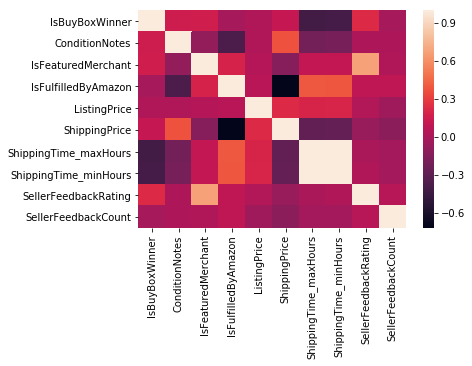
\includegraphics[width=\linewidth]{fig_market_US_corr.png}
		\caption{The U.S. \textit{"amazon.com"} market } \label{fig:corrus}
	\end{subfigure}
%	\hspace*{\fill} % separation between the subfigures
	\begin{subfigure}{0.45\textwidth}
		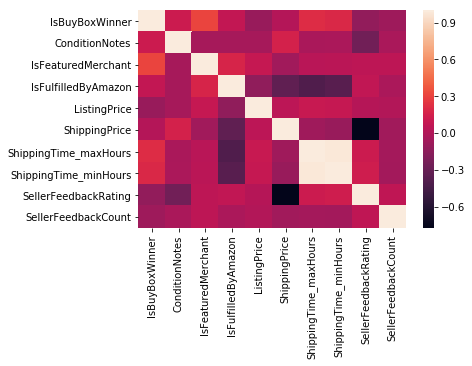
\includegraphics[width=\linewidth]{fig_market_UK_corr.png}
		\caption{The U.K. \textit{"amazon.co.uk"} market} \label{fig:corrfr}
	\end{subfigure}
	\caption{The correlation between features in (a) U.S. market and (b) U.K. market.} \label{fig:corr}
\end{figure}

In addition, we create some new features to enrich the information of an auction. These features are described as follows:

\textbf{1. Difference to Minimum Price in Auction}: (\textit{DifftoMinLandedPriceCompetition})This is the difference from current LandedPrice to the minimum landed price in that auction.

\textbf{2. Difference to the Minimum Price of Product}: (\textit{DifftoMinLandedPriceProduct}) This is the difference from current LandedPrice to the minimum landed price, grouped by product.

\textbf{3. Difference to the Amazon Seller's Price}: (\textit{DifftoAmzLandedPriceCompetition}) We capture who is the Amazon Seller in the auction. Then, we calculate the difference from current LandedPrice to the Amazon Price. If there is not Amazon Seller in the auction, we use the difference to minimum price in the auction instead.

\textbf{4. Difference to the Ideal Point in Auction}: (\textit{IdealPointCompetition}) The ideal point is the combination between the best (i.e., minimum) LandedPrice and the best (i.e., minimum) ShippingTime\_maxHours, across all offers, in each auction. This feature captures the difference from this ideal point, for each offer in the auction.
\begin{figure}[!h]
	\begin{center}
		\scalebox{0.28}{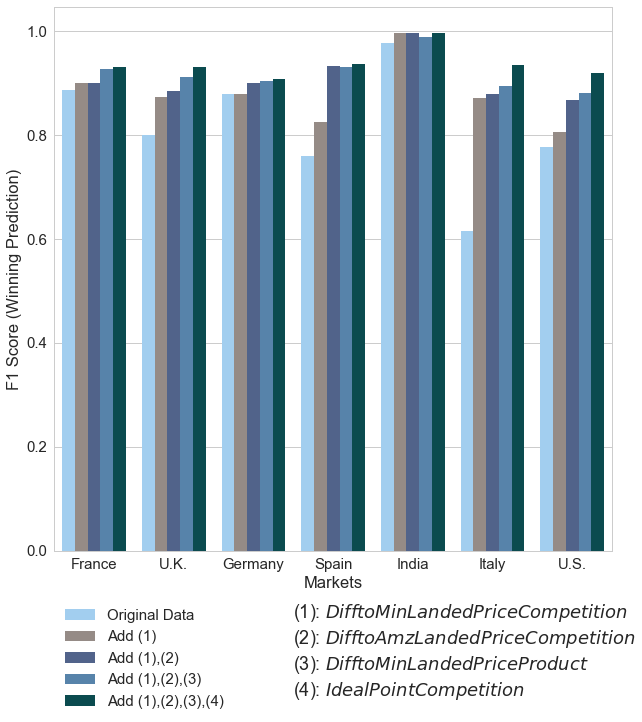
\includegraphics{fig_addFeatures.png}}
	\end{center}
	\caption{\label{fig:addfeaures}A comparison of F1-score when predicting winner BuyBox for 7 marketplaces. The scores are provided by Random Forest classifier.}
\end{figure}

%\subsubsection{Feature Selection:}
%\label{sec:featsel}
%%% This will talk about the feature importance?
%According to Amazon's documentation, as well as speculation from sellers, other
%features are possibly used by the Buy Box algorithm. 
%
%\begin{figure}[!h]
%	\begin{center}
%		\scalebox{0.27}{\includegraphics{fig7_fi.png}}
%	\end{center}
%	\caption{\label{fig:fi}An example of the Feature Importance, provided by Random Forest classifier.}
%\end{figure}

In order to check the model's improvement capability for the new features, we add those features one after another and compare them with the F1-scores by using Random Forest Classifier. \textbf{Fig.\ref{fig:addfeaures}} illustrates that the prediction becomes better when adding the extra information. This upgrading also points that the new features can enrich the Amazon data and help to build a better hypothesis.


\subsection{Machine Learning Model for Predicting BuyBox Winner}
\label{sec:buyboxmodel}

In here, we introduce the model construction with BuyBox Predictor. The goal of this algorithm is to predict the probability to win buy box. From parsed data, we use the Random Forest classifier to build the R.F. tree, which has information of who is winner and who can never win. The \textbf{Fig.\ref{fig:buyboxflow}} shows the flowchart of BuyBox prediction algorithm.

\begin{figure}[!h]
	\begin{center}
		\scalebox{0.70}{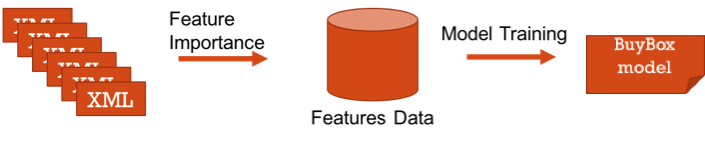
\includegraphics{fig4_buybox.png}}
	\end{center}
	\caption{\label{fig:buyboxflow}The flowchart of BuyBox model for winner prediction using feature importance to rank and select best features.}
\end{figure}

\subsection{Experiment for Predicting BuyBox Winner}
\label{sec:expbuyboxmodel}